\chapter{Thiết lập thí nghiệm và đánh giá\label{chapter:eval}}
\chaptermark{Đánh giá}

Chương này bắt đầu với các máy thử và khối lượng công việc. Kết quả rồi theo chế độ tải, rồi
theo các câu hỏi nghiên cứu còn lại.

\section{Thiết lập hệ thống thử\label{sec:testbed}}
Một số số trong chương này đến từ trình biên dịch và mã. Các số khác phụ thuộc máy chúng chạy
trên. Mọi số tốc độ ở đây đến từ một máy chủ vật lý chuyên dụng, một socket \MainCpu{}. Mỗi nhân
chạy một luồng. Đa luồng đồng thời là \MainSmt{}. Máy chạy \MainHostDistro{} trên nhân
\MainKernel{}. Linux có thể tăng và giảm xung mỗi nhân khi tải và nhiệt đổi. Xung được giữ cố
định: bộ điều tần là \MainGovernor{}, và boost tắt. Benchmark chỉ được dùng các nhân
\MainPinned{}. Không có hypervisor, nên chương trình chạy trên chính máy chứ không trong một máy
ảo. Trên các nhân đó nhân hệ điều hành tắt ngắt thời gian định kỳ (\texttt{nohz\_full}). Những
ngắt đó nếu không sẽ hiện trong các số độ trễ. Nghiên cứu không dùng \texttt{isolcpus}. Cờ đó
cũng ngăn nhân rải việc trên các nhân được phép. Mọi luồng benchmark khi đó đáp xuống một nhân.

Các trình biên dịch không phải những cái cài trên máy chủ. Cả hai bản được xây và chạy trong một
ảnh container mang \MainDistro{} với \texttt{g++~\MainGpp} và \texttt{rustc~\MainRustc}. Ảnh chốt
phiên bản chính \texttt{gcc-toolset} chứ không phải bản phát hành trong đó. Chiến dịch trước trên
một máy ảo vì vậy biên dịch với \texttt{g++~\GuestGpp}, sớm hơn một bản phát hành GNU Compiler
Collection (GCC)~15. Một container vẫn dùng nhân của máy nó ngồi trên. Hai chiến dịch khi đó
khác nhau về phần cứng, về nhân (\MainKernel{} đối với \GuestKernel{}), và về bản phát hành trình
biên dịch đó.

Cho đến muộn trong công việc, chiến dịch chạy trên một máy ảo thay vì vậy: Kernel-based Virtual
Machine (KVM) trên một \GuestCpu{}, không có các kiểm soát nhân ở trên. Trên máy đó khoảng tin
cậy $95\%$ trên p99 của một biến thể đơn trải $\GuestPNineNineMaxCI\,\mu$s, trong khi giá trị
p99 của bốn biến thể lệch $\GuestPNineNineRange\,\mu$s. Nhiễu trên một biến thể lớn hơn khoảng
cách giữa cả bốn. Chiến dịch đó được giữ. Nó dùng cùng thiết kế với chiến dịch này, nên hai bên
có thể được so để hỏi phát hiện nào thuộc về mã. Một quét thứ ba trên một máy vật lý thứ hai
\BmCpu{} dùng số phân mảnh, lưới tải, số lần lặp và trình biên dịch khác. Nó thử liệu các phát
hiện có sống sót những thay đổi đó cùng nhau, không phải từng cái tách riêng.

\section[Khối lượng và phép đo]{Khối lượng công việc và phép đo\label{sec:workload}}
Khối lượng được làm cho thí nghiệm. Các bước nó đi lấy từ quy tắc
3GPP~\cite{3gpp38401,3gpp38331}. Một bộ lái luôn gửi cùng chuỗi đưa mỗi UE qua vòng đời kết nối
mà các quy tắc đó định. Khối lượng \emph{signal} trước hết kết nối một tập UE, rồi gửi cùng thao
tác báo hiệu hết lần này đến lần khác. Điều đó cô lập đường phổ biến. Khối lượng \emph{mixed} đưa
mỗi UE qua tạo ngữ cảnh, thiết lập, báo hiệu, thiết lập bearer, tái cấu hình hoặc chuyển giao,
và giải phóng. Một thứ tự ngẫu nhiên cố định làm cả hai ngôn ngữ thấy cùng số đếm mỗi loại thao
tác cho một hạt giống cho trước. Đó cũng là một kiểm tra rằng hai bản đã làm cùng việc.
Hình~\ref{fig:workload} cho thấy hai khối lượng và chuỗi mà khối mixed đi.

\begin{figure}[ht]
\centering
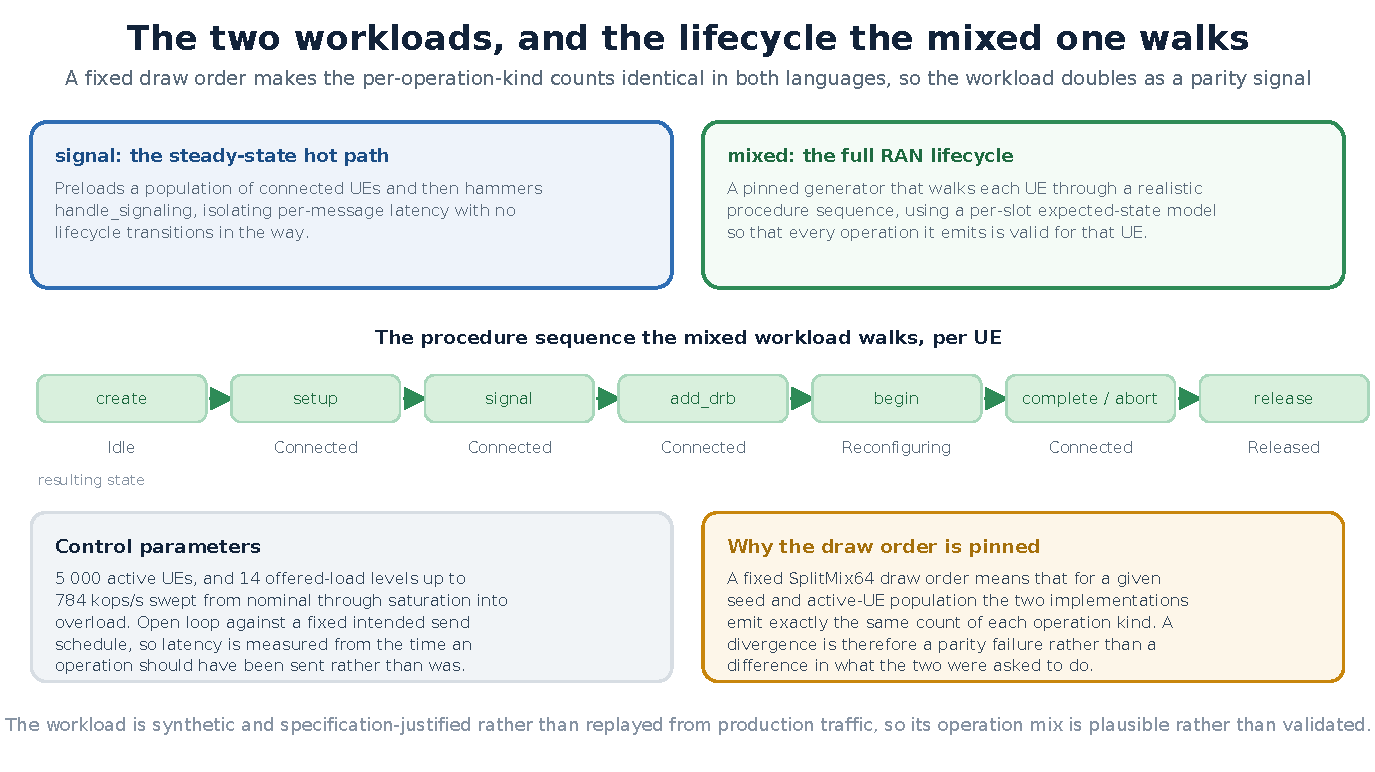
\includegraphics[width=0.78\linewidth]{diagrams/pdf/27_workload_timeline.pdf}
\caption[Hai khối lượng, và vòng đời mà khối mixed đi]{Hai khối lượng, và vòng đời mà khối mixed
đi. Signal lặp đường phổ biến, và mixed đưa mỗi UE qua chuỗi thủ tục vẽ
dưới.\label{fig:workload}}
\end{figure}

Chuỗi thao tác khớp quy tắc 3GPP. Tần suất mỗi loại xuất hiện thì không. Một cell thực chuyển
giao thường đến mức nào phụ thuộc site và giờ trong ngày, và không con số công khai nào chốt nó.
Một hỗn hợp không khớp một cell thực dịch cả hai ngôn ngữ cùng một lượng. Nó giới hạn mức các số
đi xa được. Nó không làm phép so sánh bất công. Bộ gửi giữ lịch của nó dù dịch vụ trễ (vòng hở),
và histogram được hiệu chỉnh, nên một tắc không che các trả lời thiếu (thiên lệch bỏ sót phối
hợp)~\cite{schroeder2006openclosed}. Mỗi mức tải được lặp \NRepeats{} lần. Bốn biến thể ngôn ngữ
và bộ cấp phát được đan xen trong mỗi lần lặp. Mỗi điểm báo cáo là một trung vị với khoảng tin
cậy bootstrap $95\%$~\cite{georges2007rigorous,efron1993bootstrap}.

Tải dùng cho các hình tài nguyên là $\ReprLoad$~kilo-thao-tác mỗi giây (kops/s). Đó là một giá
trị được chọn, không phải một giá trị tính từ quét. Quy tắc đầu tiên nghiên cứu này dùng là mức
tải bận nhất mà p99 ở dưới $5$~ms. Trên máy ảo quy tắc đó đáp xuống nhiễu của máy chủ. Trên một
máy yên nó leo cho đến khi dịch vụ không còn theo kịp. Nó được giữ chỉ như một kiểm tra. Cao
nguyên thông lượng thấp nhất trong bốn biến thể là $\SatKnee$~kops/s, đạt khi tải đưa vào là
$\TrackingLoad$~kops/s.

\section{Kết quả}
Các kết quả an toàn và phần lớn kết quả di trú không phụ thuộc máy nào được dùng. Các kết quả
tốc độ và bộ nhớ thì có. Mỗi hình dưới đây được đo trên máy chủ của Mục~\ref{sec:testbed} trừ
khi chú thích nói khác.

\subsection{Dưới bão hoà (RQ1, RQ3)}\label{sec:perfresults}
Khi dịch vụ vẫn theo kịp tải đưa vào, trung vị của bốn biến thể nằm trong $\PFiftyRange\,\mu$s
của nhau, $\PFiftySpread\%$. Một kiểm định ghép cặp vẫn tìm thấy khác biệt
$\PFiftyDiffAbsMax\,\mu$s nghiêng về Rust dưới cả hai bộ cấp phát. Hình~\ref{fig:loadsweep} cho
thấy quét đứng sau điều đó. Các phân vị cao hơn nay cũng đọc được. Khoảng rộng nhất trên p99 của
một biến thể đơn trải $\PNineNineMaxCI\,\mu$s. Giá trị p99 của bốn biến thể lệch
$\PNineNineRange\,\mu$s. Vì vậy nhiễu trên một cái nhỏ hơn khoảng cách giữa chúng. Trên máy ảo
cùng hai đại lượng đó là $\GuestPNineNineMaxCI\,\mu$s đối với $\GuestPNineNineRange\,\mu$s, theo
chiều ngược. Cả hai hàng p99 và cả hai hàng p99.9 vượt hiệu chỉnh Holm, \NTailSignificant{} hàng
tất cả, cùng chiều với trung vị. Bảng~\ref{tab:latency} báo cáo p99.9 và cực đại tại tải đại
diện. Cực đại được giữ ngoài họ được thử, như p99.99 gộp.

\begin{table}[ht]
\centering
\small
\caption[Độ trễ mỗi thao tác tại tải đại diện]{Độ trễ mỗi thao tác, tính bằng micro giây, tại
$\ReprLoad$~kops/s. Trung vị trên \NRepeats{} lần lặp nằm trên khoảng bootstrap $95\%$ của nó.
$^{\dagger}$Cột p99.99 được gộp giữa các lần lặp, nên không có khoảng. Cực đại được giữ ngoài họ
được thử vì cùng lý do.\label{tab:latency}}
\LatencyTabular
\hline\hline
\LatencyHead \\
\hline
C++ (system alloc) & \mci{217.2}{163.8}{237.2} & \mci{355.1}{289.3}{389.4} & \mci{674.3}{395.3}{1538.0} & \mci{2170}{910}{5594} \\
C++ (jemalloc) & \mci{225.8}{181.1}{261.2} & \mci{410.1}{305.7}{11280.4} & \mci{1188}{544}{14213} & \mci{3590}{1472}{16291} \\
Rust (system alloc) & \mci{214.3}{191.6}{238.8} & \mci{376.3}{330.2}{3629.1} & \mci{1068}{504}{6955} & \mci{2404}{1129}{9667} \\
Rust (jemalloc) & \mci{208.4}{193.7}{223.1} & \mci{388.9}{342.3}{478.0} & \mci{763.4}{479.5}{4272.1} & \mci{2804}{1114}{7606}
\\
\hline
\end{tabular}
\end{table}

\begin{figure}[ht]
\centering
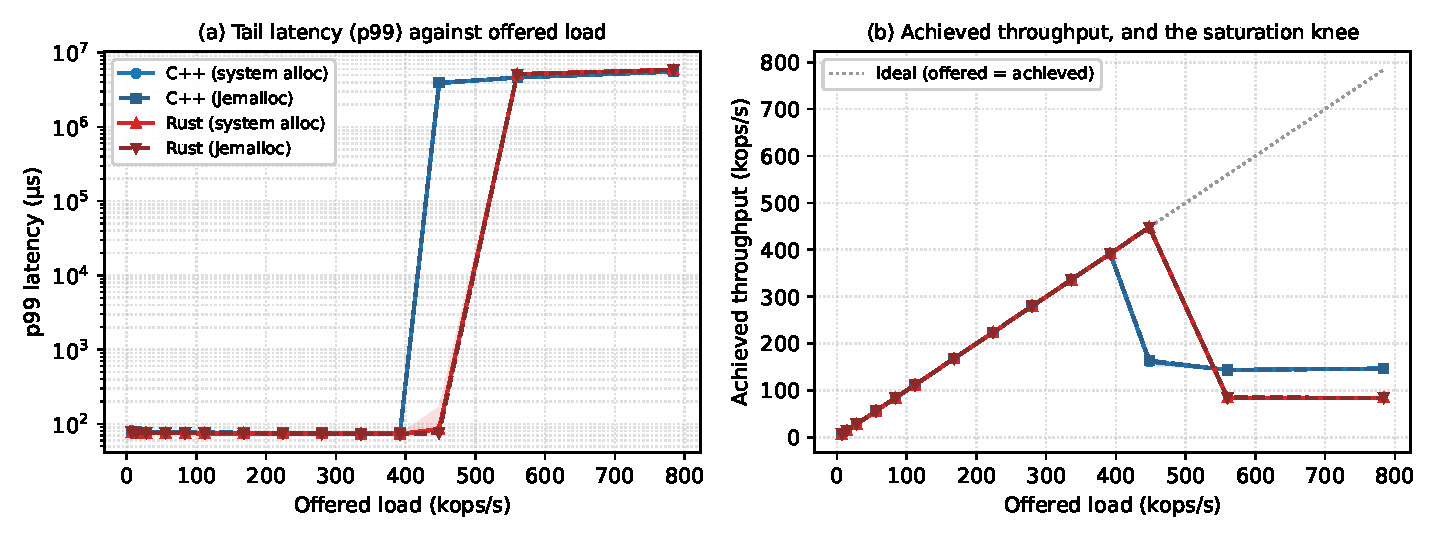
\includegraphics[width=0.78\linewidth]{figures/fig_load_sweep.pdf}
\caption[Quét tải: độ trễ đuôi và thông lượng đạt được]{Quét tải, cả hai tấm đối với tải đưa
vào. Đường là trung vị trên \NRepeats{} lần lặp, và dải là khoảng tin cậy bootstrap
$95\%$.\label{fig:loadsweep}}
\end{figure}

Đuôi xa cũng đọc được ở đây. Histogram của các lần lặp được gộp, cho \FarTailSamplesMin{} đến
\FarTailSamplesMax{} thao tác mỗi biến thể. Hai biến thể \FarTailLower{} nằm dưới cả hai biến
thể C++. Cặp rộng nhất lệch $\FarTailRange\,\mu$s. Biến thể Rust chậm nhất vẫn nằm
$\FarTailLangSep\,\mu$s dưới biến thể C++ nhanh nhất. Một máy vật lý thứ hai ở số phân mảnh khác
đồng ý, chạy $\BmFarTailCppLo$--$\BmFarTailCppHi\,\mu$s cho các biến thể C++ đối với
$\BmFarTailRustLo$--$\BmFarTailRustHi\,\mu$s cho các biến thể Rust, không chồng. Một giới hạn thứ
hai không đến từ máy. Không máy chủ nào xoá được giới hạn đó. Một vòng khứ hồi đầu-cuối chỉ dành
$\BudgetCoreShareMax\%$ thời gian cho công việc ngôn ngữ thực hiện. Phần còn lại là đưa yêu cầu
sang luồng khác, và thời gian đó được tính cho hệ điều hành. Khi công việc bên trong ngôn ngữ
nhỏ như vậy, thời gian vượt biên luồng chiếm ưu
thế~\cite{zhou2025oltp}. Quét này không thể giới hạn một hiệu ứng ngôn ngữ theo chiều nào, điều
mà Hình~\ref{fig:budget} đặt cạnh những gì quét vẫn còn cho thấy. Đo riêng, thao tác lõi nhanh
hơn $\BudgetCoreRatio\times$ ở \BudgetCoreFaster{}. Nguyên nhân khả dĩ là cách bảng băm
chuẩn được bố trí, không phải mô hình an toàn.

\begin{figure}[ht]
\centering
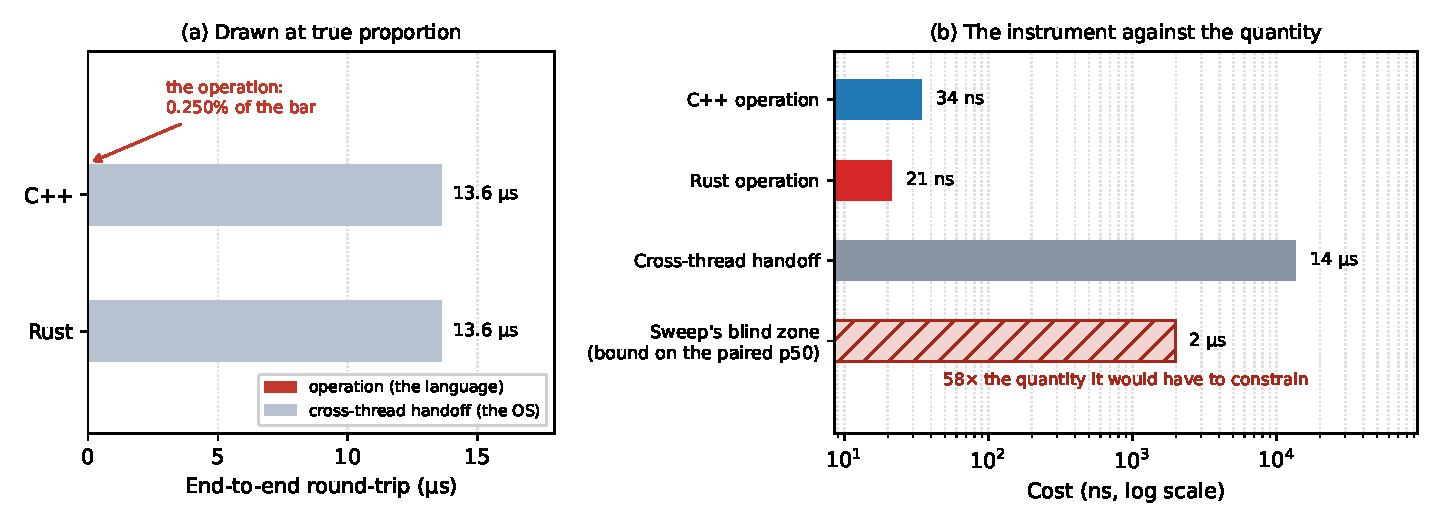
\includegraphics[width=0.78\linewidth]{figures/fig_budget.pdf}
\caption[Thao tác đầu-cuối được phân rã, đối với những gì quét phân giải được]{Chi phí của một
vòng khứ hồi đầu-cuối đi đâu. \textbf{(a)} Vòng khứ hồi ở tỉ lệ thật. \textbf{(b)} Cả hai phép
đo thao tác nằm trong vùng mù của quét theo hệ số $\BudgetBoundVsCore$.\label{fig:budget}}
\end{figure}

\subsection{Qua bão hoà (RQ1)}\label{sec:overload}
Khi tốc độ đưa vào cao hơn dịch vụ chịu được, bốn biến thể ngừng theo kịp ở các tải khác nhau.
Các bản Rust giữ đến $\TrackingLoadRust$~kops/s. Các bản C++ giữ đến $\TrackingLoadCpp$. Vì vậy
tại $\KneeGapLoad$~kops/s \KneeGapFaster{} vẫn phục vụ $\KneeGapThrFast$~kops/s nơi
\KneeGapSlower{} đã rơi xuống $\KneeGapThrSlow$. Mức tải đó được mô tả chứ không được thử, vì nó
được tìm sau khi dữ liệu đã có.

Sâu hơn, tại $\OverloadLoad$~kops/s đưa vào, thứ tự đảo. \OverloadSustainedFaster{} vẫn hoàn
thành $\OverloadThrCpp$~kops/s nơi \OverloadSustainedSlower{} hoàn thành $\OverloadThrRust$, một
hệ số $\OverloadThrRatio$, trong \OverloadThrAgree{} lần lặp dưới cả hai bộ cấp phát. Giá trị
$p$ đã hiệu chỉnh Holm nhỏ đến mức họ kiểm định này có thể đi. Biến thể chậm hơn không chỉ làm
ít việc hơn. Nó dùng $\OverloadCpuPerOpRatio$ lần CPU cho mỗi thao tác nó hoàn thành, dấu hiệu
của nỗ lực bỏ ra mà không hoàn tất gì. Khi hàng đợi bị chặn và tay cầm hoàn tất được đo riêng,
thứ tự đó không có ý nghĩa, nên nguyên nhân nằm trên đường rộng hơn đưa việc giữa các luồng.
Đây là hiệu ứng ngôn ngữ lớn nhất trong họ được thử. Một phép so sánh dừng ở tải mà dịch vụ vẫn
đáp sẽ chỉ theo chiều kia. Hình~\ref{fig:overload} đặt những gì mỗi biến thể vẫn hoàn thành cạnh
những gì nó tốn để hoàn thành.

\begin{figure}[ht]
\centering
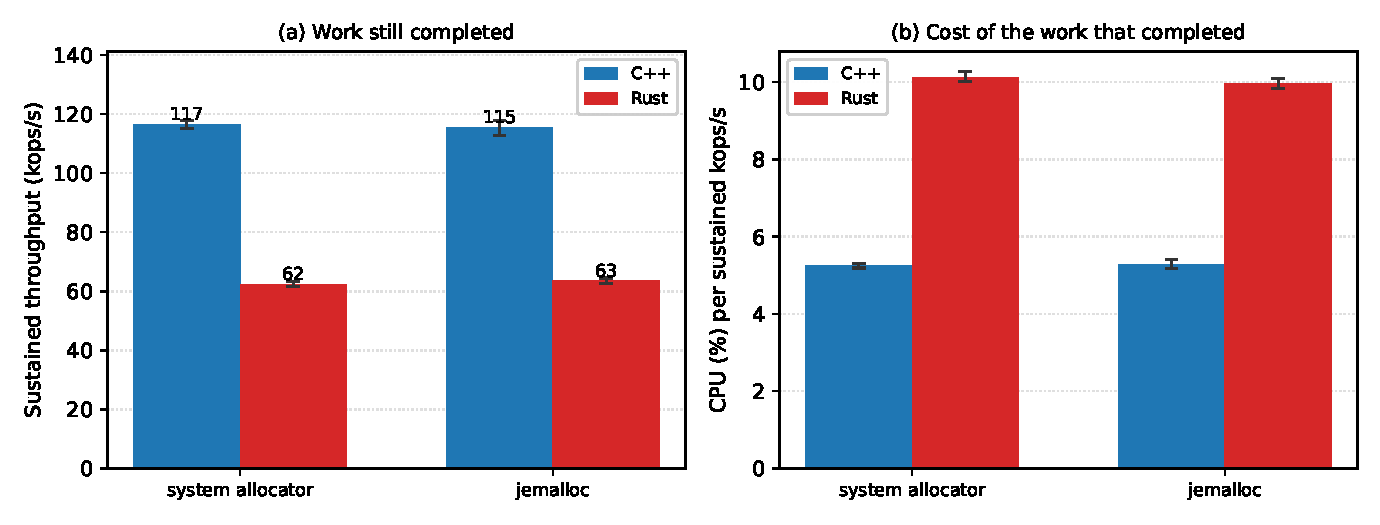
\includegraphics[width=0.78\linewidth]{figures/fig_overload.pdf}
\caption[Phân kỳ qua bão hoà]{Hành vi tại $\OverloadLoad$~kops/s đưa vào. Cột là trung vị trên
\NRepeats{} lần lặp với khoảng bootstrap $95\%$, nhóm sao cho hai cột trong một nhóm chỉ khác
ngôn ngữ. CPU trong (b) được cộng trên các luồng.\label{fig:overload}}
\end{figure}

\subsection{Dùng tài nguyên (RQ3)}\label{sec:resources}
Bộ nhớ và CPU tách các biến thể nơi độ trễ không tách được. Hai hiệu ứng cỡ tương đương nằm
trong RSS đỉnh. Bản build Rust dùng $\RssLangDiffLo$--$\RssLangDiffHi$~MiB bộ nhớ đỉnh nhiều hơn
bản build C++ dưới bộ cấp phát nào. Liên kết \texttt{jemalloc} nói chung tốn
$\RssAllocDiffLo$--$\RssAllocDiffHi$~MiB ở ngôn ngữ nào. Cả hai đều thực, và
Hình~\ref{fig:resources} đặt cặp đó cạnh RSS đỉnh mà chúng cộng thành. Hiệu ứng ngôn ngữ giữ
chiều và cỡ trên cả ba máy được đo. Của bộ cấp phát là $\GuestRssAllocOverLang$ lần hiệu ứng ngôn
ngữ trên máy ảo nghiên cứu này dùng trước ($\GuestRssAllocLo$--$\GuestRssAllocHi$~MiB), nên tỉ
số của chúng phụ thuộc máy. Khác biệt ngôn ngữ là chi phí cố định, không phải chi phí mỗi UE.
Máy yên là nơi điều đó nhìn thấy được. Bộ đếm của chính \texttt{jemalloc} ở đó đặt
$\BmJeMetadataDelta$~MiB nhiều hơn vào sổ sách arena và $\BmJeAllocatedDelta$~MiB \emph{ít hơn}
vào cấp phát còn sống. Byte trú của nó thấp hơn $\BmJeResidentDelta$~MiB. Đỉnh tiến trình cao
hơn $\BmJeRssDelta$~MiB. Bộ nhớ thêm khi đó nằm ngoài bộ cấp phát, trong thời gian chạy mà một
tiến trình Rust mang trước khi nó cấp phát. CPU đổi dấu theo tải. Tại tải đại diện
$\ReprLoad$~kops/s Rust dùng ít hơn tối đa $\CpuDiffAbsMax$ điểm phần trăm. Khi dịch vụ không
còn theo kịp, CPU mỗi thao tác hoàn thành cao hơn nhiều.

\begin{figure}[ht]
\centering
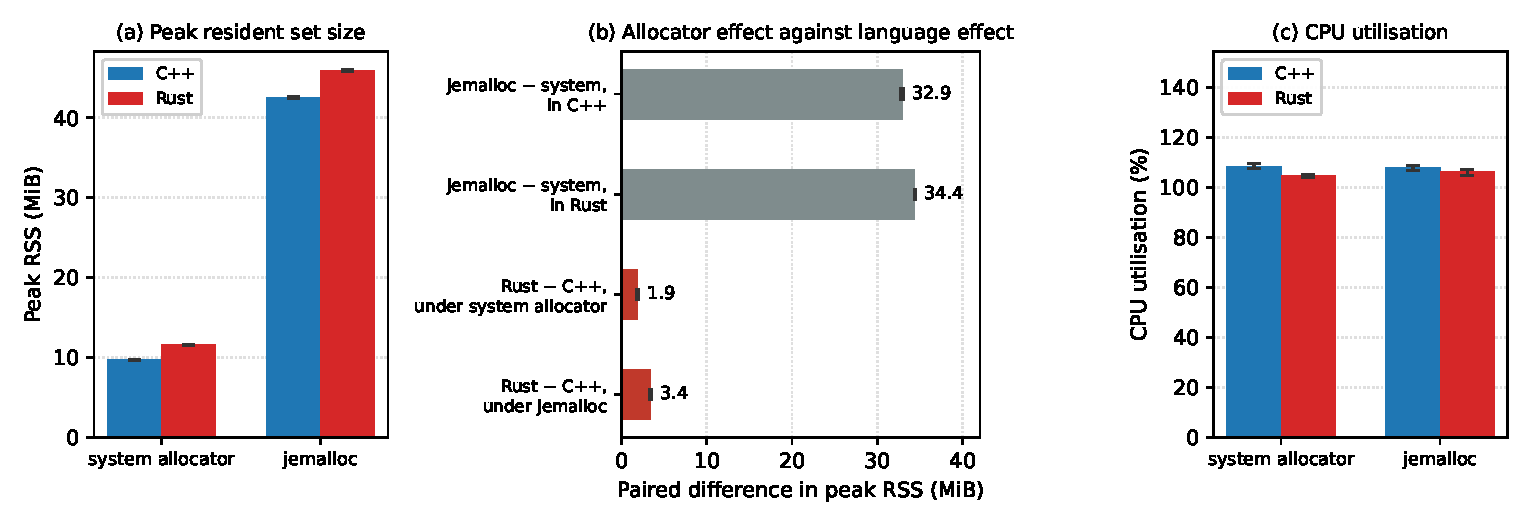
\includegraphics[width=0.78\linewidth]{figures/fig_resources.pdf}
\caption[Dùng tài nguyên, và hai hiệu ứng trong RSS đỉnh]{Dùng tài nguyên tại
$\ReprLoad$~kops/s, nhóm theo bộ cấp phát. Cột là trung vị trên \NRepeats{} lần lặp với khoảng
bootstrap $95\%$, và CPU trong (c) được cộng trên các luồng.\label{fig:resources}}
\end{figure}

\subsection{An toàn qua tiêm lỗi (RQ2)}\label{sec:safetyresults}
An toàn được đo bằng cách tiêm $\FaultClasses$ lỗi. Bảy lớp đến từ bên trong vùng Rust tuyên bố
cai quản. Bảy lớp được chọn vì Rust an toàn được kỳ vọng \emph{không} ngăn chúng. Mỗi lớp trong
bảy lớp đầu là lỗi biên dịch ở Rust. Ở C++ mỗi lớp là mã hợp lệ. Lỗi chỉ hiện nếu một kiểm thử
đưa nó chạy, và không bộ dò lỗi đơn nào phủ chúng. Use-after-move là trường hợp không bộ dò lỗi
nào báo gì. Một đối tượng đã move vẫn là một đối tượng hợp lệ. Giá trị của nó không xác định.
Vì vậy không có gì bất hợp pháp để phát hiện, và định danh đơn giản là mất. Cả bảy trường hợp
biên đều biên dịch trong Rust an toàn và hành xử sai. Trên hai lớp trong số đó công cụ C++ là
bên báo. LeakSanitizer gắn cờ chu trình tham chiếu mà Rust rò trong im lặng, vì rò là an toàn
trong Rust theo thiết kế tường minh~\cite{hughes2025gcrust,cui2024rcanary}.
UndefinedBehaviorSanitizer gắn cờ overflow mà Rust định nghĩa là quấn. ThreadSanitizer bắt đảo
thứ tự khoá trong $\DeadlockTsanHits$ trên $\DeadlockTsanRuns$ lần chạy, một tỉ lệ bản thân không
ổn định. Nó chỉ ghi thứ tự khoá từ các khoá thành công. Nếu lần đảo đầu chờ mãi, chu trình không
bao giờ đóng, nên công cụ không bao giờ báo.

Double-free đường nối là double-free trong bảo đảm viết lại qua \texttt{unsafe}, không phải một
lớp mới. Nửa C++ của nó không đổi, nên chỉ cột Rust dịch. Hai bộ kiểm tra mô hình Rust có báo cả
hai lỗi biên gốc. Loom duyệt xen kẽ luồng một cách vững. Shuttle lấy mẫu những xen kẽ Loom không
với tới~\cite{bornholt2021shardstore}. Mỗi cái phải được viết bằng nguyên thủy của chính bộ kiểm
tra trước, và thu nhỏ về cỡ mô hình. Miri báo double-free đường nối, nhưng nó diễn giải Rust và
không chạy được máy chủ C++ mà lỗi nằm sau. LeakSanitizer và UndefinedBehaviorSanitizer báo mà
không cần viết lại. Hai bộ kiểm tra mô hình chỉ báo các trường hợp biên tương tranh sau khi lỗi
được viết lại vào nguyên thủy của chúng. Hình~\ref{fig:taxonomy} vẽ cả danh mục như một ma trận
kết cục. Resource Acquisition Is Initialization (RAII) gỡ việc quên mở khoá thông thường. Nó không
gỡ lớp: cả hai chương trình quên guard đều treo, và công cụ của ngôn ngữ nào cũng không nói vậy.

\begin{figure}[ht]
\centering
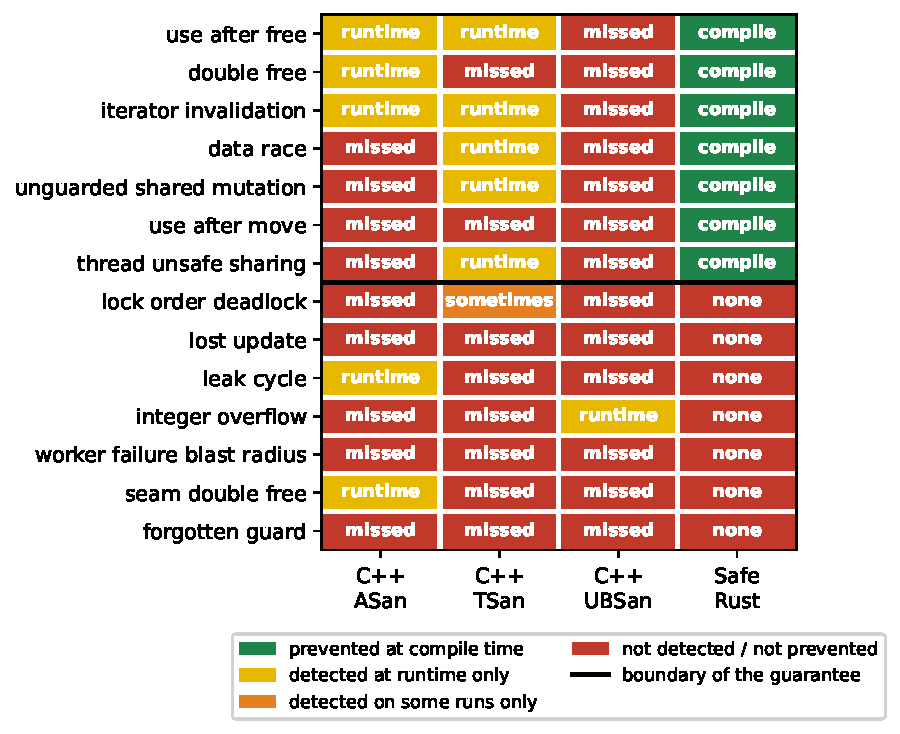
\includegraphics[width=0.72\linewidth]{figures/fig_taxonomy.pdf}
\caption[Nơi bảo đảm dừng: ma trận kết cục]{Kết cục tiêm lỗi như một ma trận, sinh từ nhật ký
phân loại.\label{fig:taxonomy}}
\end{figure}

\subsection{Di trú (RQ4)}\label{sec:migrationresults}
Đường nối di trú nhỏ trên mỗi trục được đo: $\FfiEntryPoints$ điểm vào C trong $\FfiSeamLines$
dòng Rust. Mọi việc con trỏ thô bị nhốt trong $\FfiUnsafeFns$ hàm. Lõi được để không
\texttt{unsafe}. Không chi phí thêm nào được phát hiện đối với cùng cuộc gọi báo hiệu thực hiện
trực tiếp. Điều đó giới hạn mọi thuế mỗi lần gọi ở $\FfiOpBoundPct\%$ của cuộc gọi đó, và
Hình~\ref{fig:ffiseam} cho thấy cấu trúc mà giới hạn đó thuộc về. Ba chi phí áp dụng ngoài đường
nối cũng được đo, và hai trong số đó mâu thuẫn với phản đối thường gặp khi áp dụng Rust.
$\BuildDepShareCpu\%$ của lần build sạch Rust là mã bên thứ ba. Mã nguồn của chính dự án biên
dịch trong $\BuildAllFirstPartyCpuRatio$ lần CPU mà \texttt{g++} cần. Khoảng cách kích thước nhị
phân $\FootShippedRatio\times$ là một chính sách liên kết đảo chiều khi chính sách được giữ cố
định. Thành phần được so sánh không có crate bên thứ ba và không có vị trí \texttt{unsafe}
($\DepsCore$ crate, $\CoreUnsafe$ vị trí \texttt{unsafe}).

\begin{figure}[ht]
\centering
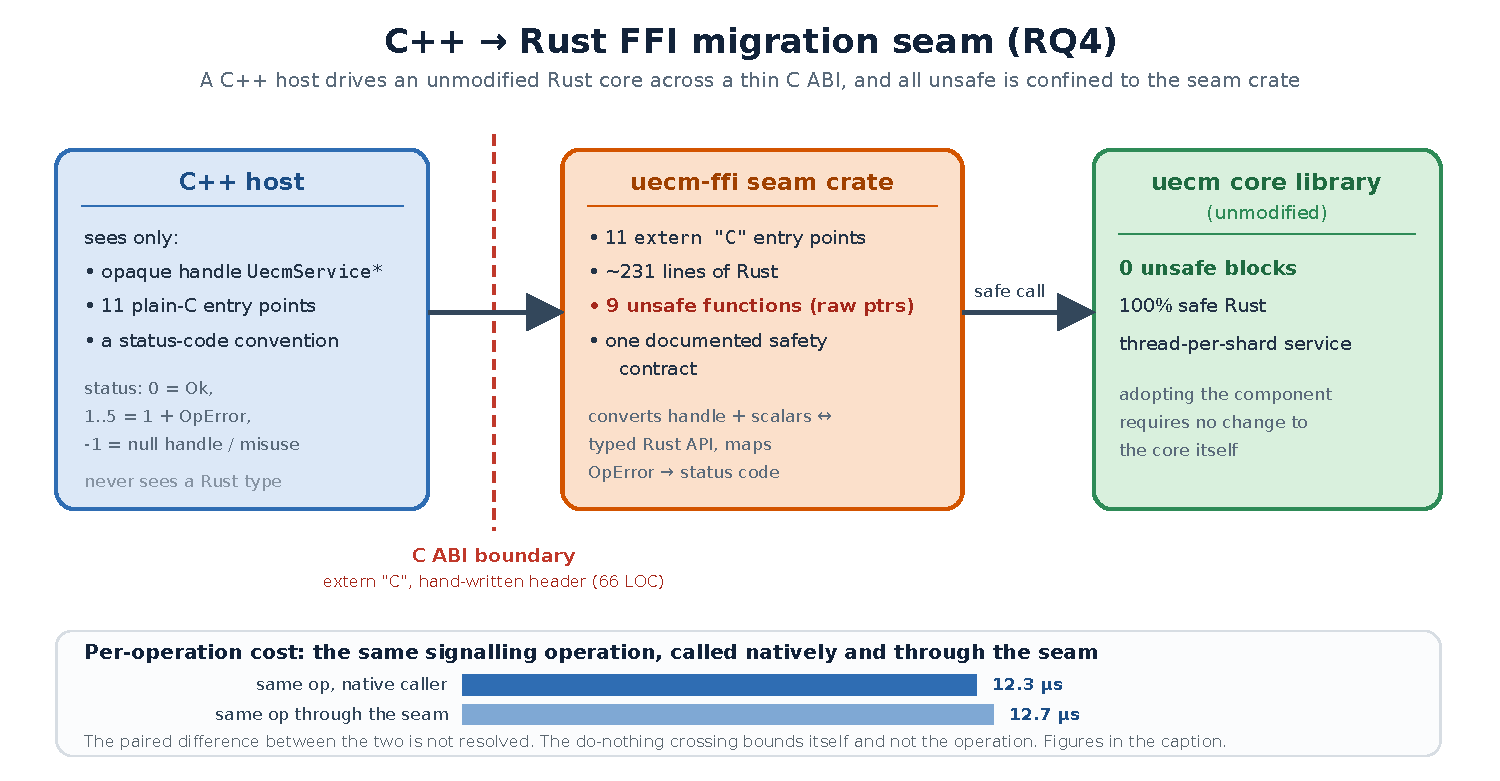
\includegraphics[width=0.78\linewidth]{diagrams/pdf/07_ffi_seam.pdf}
\caption[Đường nối di trú FFI từ C++ sang Rust]{Đường nối di trú FFI từ C++ sang Rust. Cùng thao
tác báo hiệu tốn $\FfiOpNative$~\textmu s trực tiếp và $\FfiOpSeam$~\textmu s qua đường nối, một
khác biệt ghép cặp được giới hạn ở $\FfiOpBoundPct\%$ của cuộc gọi đó. Một lần vượt không làm gì
tốn $\FfiCrossing$~ns và chỉ giới hạn chính nó.\label{fig:ffiseam}}
\end{figure}
